%This is part of Un soupçon de mathématique sans être agressif pour autant
% Copyright (c) 2012-2013
%   Laurent Claessens, Pauline Klein
% See the file fdl-1.3.txt for copying conditions.

% Ce fichier contient un peu plein de trucs que j'ai fait sur les fonctions et qui ne servent plus ou pas encore.


Les figures \ref{LabelFigFnAffineipcEQfssLabelSubFigFnAffineipcEQf0} et \ref{LabelFigFnAffineipcEQfssLabelSubFigFnAffineipcEQf1} montrent des droites affines. Lorsque \( m>0\), la droite monte; lorsque \( m<0\) elle descend. La pente est d'autant plus forte que \( m\) est grand.
\newcommand{\CaptionFigFnAffineipcEQf}{Deux droites affines.}
\input{Fig_FnAffineipcEQf.pstricks}

%---------------------------------------------------------------------------------------------------------------------------
\section{Résolution graphique d'(in)équations} 
%---------------------------------------------------------------------------------------------------------------------------

\subsection{Lecture graphique des images et des antécédents}

\begin{multicols}{2}

    Nous considérons la fonction
    \begin{equation}
        \begin{aligned}
            f\colon \eR&\to \eR \\
            x&\mapsto x^2 
        \end{aligned}
    \end{equation}
    dont le graphe est donné ci-contre. À chaque réel $x$, nous associons l'abscisse $y=f(x)$.  À l'aide du graphe donné, répondre aux questions suivantes.

    \begin{itemize}
        \item Image de $1,5$ ? 
        \item Antécédent de $3,5$ ?  
        \item Antécédent de $-1$ ? 
        \item Antécédent de $0$ ? 
    \end{itemize}

    \columnbreak

    %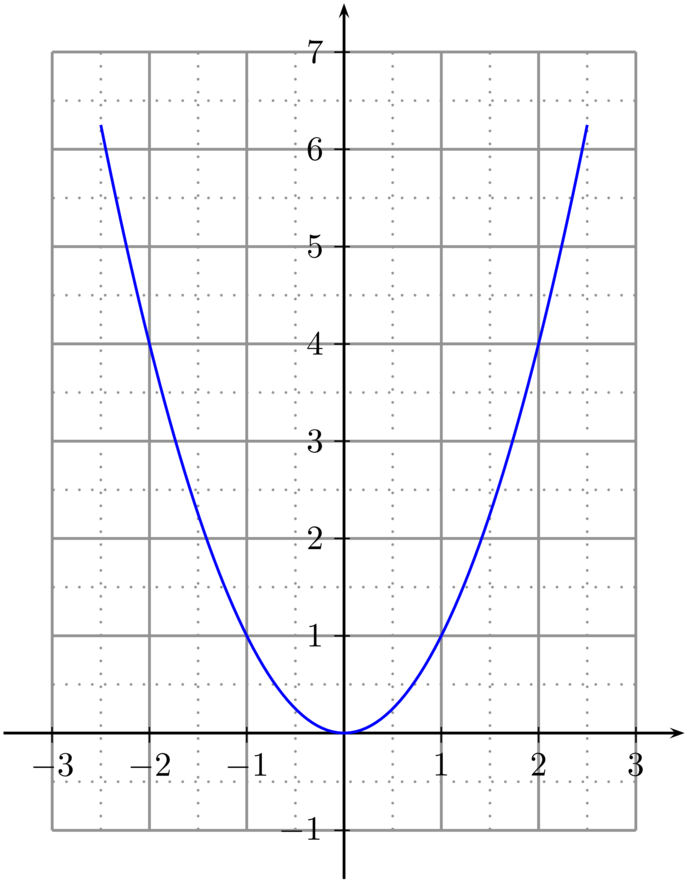
\includegraphics{Picture_FIGLabelFigFCarreQFhsWzPICTFCarreQFhsWz-for_eps.pdf}
    %\newcommand{\CaptionFigFCarreQFhsWz}{Le graphe de la fonction \( x\mapsto x^2\).}
    \input{Fig_FCarreQFhsWz.pstricks}

\end{multicols}

  \begin{example}
Compléter le tableau suivant pour la fonction $f(x)=x^2$.
\begin{equation}
\begin{array}[h]{|c|c|c|c|c|c|c|c|c|c|c|c|}
  \hline  
  x & -4 & -3 & -2 & -1 & 0 & 1 & 2 & 3 & 4 & -0,5 & 0,5  \\
  \hline
  y & 16 &&&&&&&&&&0.25\\
  \hline
\end{array}
\end{equation}
  \end{example}


\subsection{Résolution graphique d'équations}

\begin{Aretenir}
    Soit $k$, un réel fixé. Résoudre l'équation $f(x)=k$ revient à chercher les antécédents par $f$ du nombre $k$.

Le nombre de solutions de l'équation $f(x)=k$ est égal au nombre de points d'intersection de la courbe représentative de \( f\) avec la droite $d$ d'équation $y=k$. Les solutions sont les abscisses de ces points d'intersection. 
\end{Aretenir}


\begin{example}
    \begin{multicols}{2}
  Nous cherchons à résoudre $f(x)=4$. 
  \begin{itemize}
      \item 
          Nous traçons la droite horizontale d'équation \( y=4\);
      \item
          nous observons les points d'intersection de cette droite avec la courbe;
      \item
          les solutions de l'équation sont les abscisses de ces points.
  \end{itemize}

\columnbreak


%The result is on figure \ref{LabelFigExCarrexvfvre}. % From file ExCarrexvfvre
%\newcommand{\CaptionFigExCarrexvfvre}{<+Type your caption here+>}
\input{Fig_ExCarrexvfvre.pstricks}

    \end{multicols}

    Sans surprises, les solutions de \( x^2=4\) sont \( x=2\) et \( x=-2\).

\end{example}



%///////////////////////////////////////////////////////////////////////////////////////////////////////////////////////////
\subsubsection{Inéquation du type $f(x)<g(x)$}
%///////////////////////////////////////////////////////////////////////////////////////////////////////////////////////////

Les solutions de l'inéquation $f(x)<g(x)$ sont les abscisses des points pour lesquels la courbe de \( f\) est en-dessous de la courbe de \( g\).

\newcommand{\CaptionFigExIneqfgZWStde}{En cyan, l'ensemble des solutions de l'inéquation \( f(x)<g(x)\).}
\input{Fig_ExIneqfgZWStde.pstricks}

La figure \ref{LabelFigExIneqfgZWStde} montre la résolution d'une telle inéquation. Notons que l'ensemble des solutions peut être en plusieurs morceaux.

\subsection{Tableau de variations}


Le \defe{tableau de variation}{tableau de variation} est un tableau contenant
\begin{enumerate}
    \item
        les positions des sommets,
    \item
        les flèches indiquant les endroits où la fonction est croissante ou décroissante.
\end{enumerate}
Un petit exemple valant mieux qu'un long discours\ldots

% à noter le 9 dans l'environnement suivant est le nombre de lignes sur lesquelles la figure s'étale. Je suis obligé de donner à la main parce que le tableau ne compte apparemment que pour une seule ligne. Du coup si je laisse à LaTeX le soin de calculer, les lignes de texte en-dessous de la figure (et en particulier à la page suivante si la figure est en bas de page) sont encore coupées.
\begin{wrapfigure}[9]{r}{6.0cm}     
   \vspace{-1cm}        % à adapter.
   \centering
   \input{Fig_GrapheVarREGMqx.pstricks}
\end{wrapfigure}

    Le tableau de variation de la fonction dessinée ci-contre est :
    \begin{equation*}
    \begin{array}[h]{|c|ccccccc|}
        \hline
        x&-3&&-2&&0&&2\\
        \hline
        &&&2&&&&1\\
        f(x)&&\nearrow&&\searrow&&\nearrow&\\
        &-\frac{ 9 }{2}&&&&-\frac{ 1 }{2}&&\\
        \hline
    \end{array}
    \end{equation*}
    En effet, la fonction \( f\)
    \begin{itemize}
        \item 
            part de \( x=-3\) où \( f(x)=-9/2\);
        \item
            elle monte jusqu'en \( x=-2\) où elle vaut \( f(x)=2\);
        \item
            elle descend jusqu'en \( x=0\) où elle vaut \( -\frac{ 1 }{2}\);
        \item
            elle monte jusqu'en \( x=2\) où elle vaut \( 1\).
    \end{itemize}

Le plus souvent si on donne un dessin, les nombres à placer dans un tableau de variation sont des valeur approchées à la précision du dessin. Donner les réponses en fraction n'est donc pas obligatoire. Par exemple ici au lieu d'écrire \( -9/2\) dans le tableau, il aurait été possible d'écrire \( -4.5\).

\section{Minimum et maximum}

Les notions de minima et maxima parlent, comme l'indiquent leurs noms en français, des points du graphe d'une fonction les plus hauts et les plus bas.

\begin{definition}
      Soit $f$ une fonction définie sur un intervalle $I$.
      \begin{itemize}
          \item On dit que $f$ admet le réel $m$ pour \defe{minimum}{minimum (d'une fonction)} sur $I$ si et seulement si il existe $c\in I$ tel que $f(c)=m$ et pour tout $x\in I$, $f(x)\geq m$. 
    \item On dit que $f$ admet le réel $M$ pour \defe{maximum}{maximum} sur $I$ si et seulement si il existe $d\in I$ tel que $f(d)=M$ et pour tout $x\in I$, $f(x)\leq M$.
      \end{itemize}
\end{definition}

%Sur la figure \ref{LabelFigMinMaxKNRdOd}, nous avons indiqué le minimum et le maximum de la fonction dessinée.
%\newcommand{\CaptionFigMinMaxKNRdOd}{Minimum et maximum d'une fonction.}
Sur le dessin ci-dessous nous avons indiqué le minimum et le maximum de la fonction dessinée.
\input{Fig_MinMaxKNRdOd.pstricks}

%+++++++++++++++++++++++++++++++++++++++++++++++++++++++++++++++++++++++++++++++++++++++++++++++++++++++++++++++++++++++++++ 
\section{Pour tracer}
%+++++++++++++++++++++++++++++++++++++++++++++++++++++++++++++++++++++++++++++++++++++++++++++++++++++++++++++++++++++++++++

Quelque conseils pour dessiner.
\begin{itemize}
    \item
        Pour une valeur $x$ sur l'axe des abscisses, il y a un et un seul point d'abscisse $x$ sur la courbe.
    \item
        Pour tracer une courbe, il faut placer des points. Plus on choisit de points, plus la courbe sera précise.
    \item
        Si possible, trouver quelque valeurs clefs. Par exemple on cherchera les points d'intersection entre les axes et les courbe. Le point \( (0,f(0)) \) est intéressant à mettre, ainsi que les points \( x\) tels que \( f(x)=0\).
\end{itemize}


\newcommand{\CaptionFigExFonction}{Comment tracer la fonction \( f\colon x\to 2x+1\) ?}
\input{Fig_ExFonction.pstricks}

Nous donnons à la figure \ref{LabelFigExFonction} le tracé de la fonction \( f(x)=2x+1\). La figure \ref{LabelFigExFonctionssLabelSubFigExFonction0} donne quelque points du graphe de la fonction. La figure \ref{LabelFigExFonctionssLabelSubFigExFonction1} donne le graphe complet de la fonction. Comment le construit-on ? Par définition pour chaque \( x\) sur l'axe des abscisses (il y en a une infinité), il faut calculer le nombre \( f(x)\) et mettre dans le plan le point de coordonnées \( \big( x,f(x) \big)\).

En pratique, il n'est pas possible de calculer \( f(x)\) pour \emph{tous} les \( x\) réels\footnote{Chuck Norris peut le faire.}. C'est pourquoi nous nous contentons qu'en calculer quelque uns, et nous les relions «le plus intelligemment possible».


%---------------------------------------------------------------------------------------------------------------------------
\subsection{Ce qui n'est pas une fonction}
%---------------------------------------------------------------------------------------------------------------------------

%    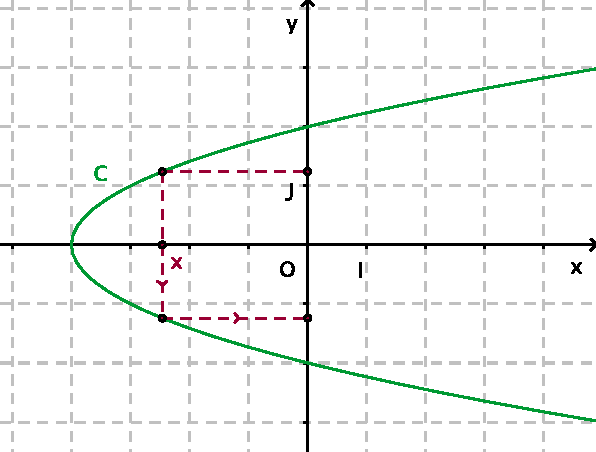
\includegraphics[width=5cm]{F_NonFct.pdf}

\begin{multicols}{2}
    Cette courbe ne représente pas une fonction, car à partir de \( x=-4\), les nombres ont deux images. Les courbes données par des fonctions sont des courbes acceptant une seule ordonnée pour chaque abscisse.

\columnbreak

%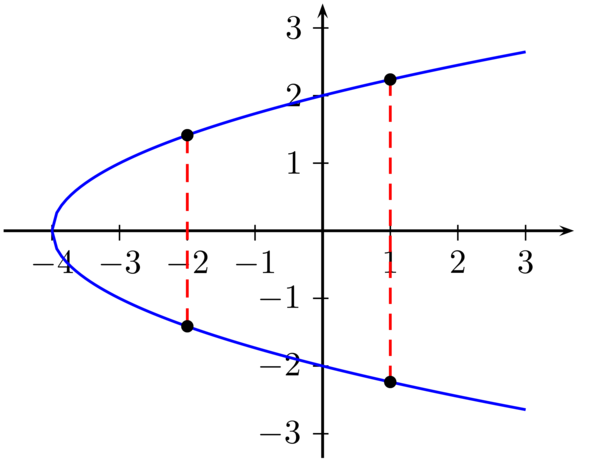
\includegraphics{Picture_FIGLabelFigPasFonctionYoQfSuPICTPasFonctionYoQfSu-for_eps.pdf}

\input{Fig_PasFonctionYoQfSu.pstricks}

\end{multicols}


Pour tracer le graphe d'une fonction affine.
\begin{itemize}
    \item
        Vu que le graphe est une droite, il suffit de deux points.
    \item
        Les fonction linéaires passent par l'origine \( (0;0)\).
    \item 
        Pour un tracé à la règle, il est plus précis de prendre deux points relativement éloignés.
    \item
        La droite \( f(x)=mx+p\) monte si \( m>0\) et descend si \( m<0\). La pente est d'autant plus forte que \( m\) est grand.
\end{itemize}

Quelque exemples à la figure \ref{LabelFigGrapheAffinHqXJGx}.
\newcommand{\CaptionFigGrapheAffinHqXJGx}{Des graphes de fonctions linéaires et affines.}
\input{Fig_GrapheAffinHqXJGx.pstricks}
%+++++++++++++++++++++++++++++++++++++++++++++++++++++++++++++++++++++++++++++++++++++++++++++++++++++++++++++++++++++++++++
\section{Modélisation par une fonction}
%+++++++++++++++++++++++++++++++++++++++++++++++++++++++++++++++++++++++++++++++++++++++++++++++++++++++++++++++++++++++++++

Les exemples de fonctions dans la «vraie» vie sont nombreux.

\begin{example}
    Soit un triangle rectangle isocèle dont les côtés de l'angle droit sont de longueur \( x\). Alors la surface est donnée par la fonction
    \begin{equation}
        f(x)=\frac{ x^2 }{2}.
    \end{equation}
    L'ensemble de définition est \( \defD=\mathopen] 0 , \infty \mathclose[\) parce que \( x\) représente une longueur.
\end{example}

\begin{example}
    Un vélo se déplace à \( \unit{20}{\kilo\meter\per\hour}\). Après un temps \( t\), il aura parcouru une distance
    \begin{equation}
        d(t)=20t
    \end{equation}
    kilomètres. Ici l'ensemble de définition est plus délicat; il dépend du contexte.

    Notons que la variable d'une fonction n'est pas obligatoirement toujours notée \( x\) et que la fonction n'est pas toujours obligatoirement notée \( f\).
\end{example}

\begin{example}
    Vous verrez dans un cours de physique que si on lance un objet verticalement avec une vitesse initiale \( v_0\), alors la hauteur en fonction du temps est donnée par
    \begin{equation}
        h(t)=v_0t-\frac{ gt^2 }{2}
    \end{equation}
    où \( g\) est l'accélération de la gravitation sur Terre (environ \( \unit{10}{\meter\per\second\squared}\)).
\end{example}

\section{Sens de variation d'une fonction}

\subsection{Notion intuitive}

\begin{multicols}{2}

    La fonction ci-contre descend jusqu'à \( -2.5\) puis monte entre \( -2.5\) et \( 2\) pour ensuite descendre.

    Nous disons qu'elle est
    \begin{itemize}
        \item 
            \emph{décroissante} sur \( \mathopen] \infty , -2.5 \mathclose]\);
        \item
            \emph{croissante} sur \( \mathopen[ -2.5 , 2 \mathclose]\);
        \item
            à nouveau décroissante sur \( \mathopen[ 2 , \infty [\).
    \end{itemize}
    
    \columnbreak

\input{Fig_ExVariationRXTkoc.pstricks}

\end{multicols}


\begin{definition}
    On dit que $f$ est \defe{strictement croissante}{strictement croissante} sur~$I$
  si pour tous réels $a$ et $b$ de $I$ tels que $a<b$, on a $f(a)<f(b)$.

  La fonction \( f\) est \defe{strictement décroissante}{strictement décroissante} sur \( I\) si pour tous réels $a$ et $b$ de $I$ tels que $a<b$, on a $f(a)>f(b)$.
\end{definition}
La différence entre la croissance et la \emph{stricte} croissance est que l'inégalité est stricte.

\begin{definition}
    Soit \( I\) un intervalle de \( \eR\). Nous disons que la fonction \( f\) est \defe{monotone}{monotone} sur $I$ si elle est soit croissante sur $I$, soit décroissante sur $I$.
\end{definition}

\begin{multicols}{2}
    La fonction dessinée ci-contre n'est pas monotone sur l'intervalle \( \mathopen[ -2 , 0 \mathclose]\). Elle est
    \begin{itemize}
        \item 
            monotone décroissante sur \( \mathopen[ -2.5 , -1 \mathclose]\);
        \item
            monotone croissante sur \( \mathopen[ -1 , 1 \mathclose]\);
        \item
            monotone décroissante sur \( \mathopen[ 1 , 1.5 \mathclose]\).
    \end{itemize}
\columnbreak
\input{Fig_GrapheVarndvdQM.pstricks}
\end{multicols}

\begin{definition}
    Soit \( I\) un intervalle. On dit que $f$ est \defe{constante}{constante (fonction)} sur $I$ lorsque pour tous les réels $a$ et $b$ de $I$, on a $f(a)=f(b)$. (Tous les réels de $I$ ont la même image par $f$).
\end{definition}

\begin{multicols}{2}
    Dans ce cas, il existe $k\in\eR$ tel que pour tout $a\in I$, $f(a)=k$. 
    
    La figure ci-contre donne le graphe de la fonction \( f(x)=1.5\) entre \( x=-3\) et \( x=3\).

\columnbreak

%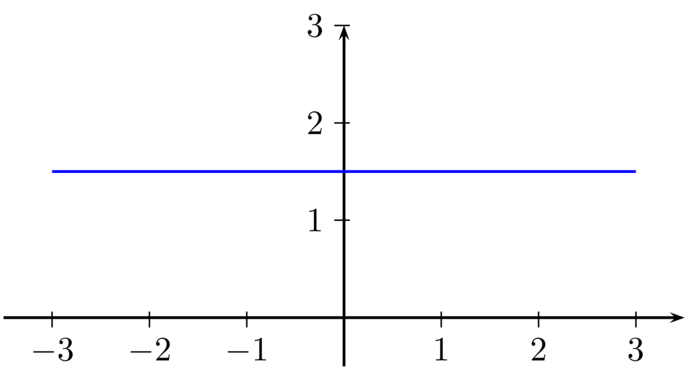
\includegraphics{Picture_FIGLabelFigFoncConstFdDkhWPICTFoncConstFdDkhW-for_eps.pdf}
%The result is on figure \ref{LabelFigFoncConstFdDkhW}.
%\newcommand{\CaptionFigFoncConstFdDkhW}{<+Type your caption here+>}
\input{Fig_FoncConstFdDkhW.pstricks}

\end{multicols}



\begin{wrapfigure}{r}{7.0cm}
   \vspace{-0.5cm}        % à adapter.
   \centering
   \input{Fig_figureCFoZCYe.pstricks}
\end{wrapfigure}

    Sur la figure ci-contre, nous avons tracé les graphes des fonctions données par
    \begin{enumerate}
        \item
            \( f(x)=2x+1\)
        \item
            \( g(x)=2x-2\)
        \item
            \( h(x)=3x-1\)
    \end{enumerate}


Nous constatons que
\begin{enumerate}
    \item
        Les droites représentatives de \( f\) et \( g\) sont parallèles.
    \item
        La droite \( h\) est plus pendue que les deux autres.
\end{enumerate}


\begin{example}
    Soit la fonction \( f(x)=3x-1\).
    \begin{enumerate}
        \item
            Le point \( (0;-1)\) est sur la courbe représentative de \( f\) parce que \( f(0)=1\).
        \item
            Le point \( (10;29)\) est également sur la courbe parce que \( f(10)=29\).
        \item
            Le point \( (2;3)\) n'est par contre pas sur le graphe parce que \( f(2)=5\neq 4\).
    \end{enumerate}
\end{example}

%+++++++++++++++++++++++++++++++++++++++++++++++++++++++++++++++++++++++++++++++++++++++++++++++++++++++++++++++++++++++++++
\section{Petit tour de magie}
%+++++++++++++++++++++++++++++++++++++++++++++++++++++++++++++++++++++++++++++++++++++++++++++++++++++++++++++++++++++++++++

\begin{Aprojeter}
    \begin{example} \label{ExemVmCkIH}
        Un petit tour de magie. Choisissez un nombre entre \( 1\) et \( 10\). Ajoutez \( 5\), multipliez par \( 2\), ajoutez \( 7\), enlevez le double du nombre de départ.
    \end{example}
\end{Aprojeter}

\begin{Aprojeter}
    Pouvez-vous trouver un petit tour de magie qui commence par
    \begin{itemize}
        \item Multiplier par \( 3\)
        \item Faire \( +2\)
        \item \ldots
    \end{itemize}
    et qui donne toujours \( 5\) ?
\end{Aprojeter}

\begin{Aprojeter}
    \lstinputlisting{ex_algo18.py}
\end{Aprojeter}


%+++++++++++++++++++++++++++++++++++++++++++++++++++++++++++++++++++++++++++++++++++++++++++++++++++++++++++++++++++++++++++ 
\section{Ensemble de définition}
%+++++++++++++++++++++++++++++++++++++++++++++++++++++++++++++++++++++++++++++++++++++++++++++++++++++++++++++++++++++++++++

\begin{definition}
    Soit \( \defD\) un ensemble de nombres. On définit une \defe{fonction}{fonction} \( f\) sur \( \defD\) en associant à chaque nombre \( x\) dans \( \defD\) un seul nombre \( y\). Dans ce cas nous disons que \( f\) est une fonction de la \defe{variable}{variable} \( x\).
\end{definition}

\begin{example}
    Soit la fonction qui à la longueur d'un segment fait correspondre la surface du carré construit sur ce segment. Cette fonction n'est définie que sur les nombres positifs (parce qu'il n'existe pas de segments de longueurs négatives). Nous écrivons donc
    \begin{equation}
        \begin{aligned}
            f\colon \mathopen[ 0 , \infty [&\to \eR \\
            x&\mapsto x^2,
        \end{aligned}
    \end{equation}
    et nous avons \( f(x)=x^2\).

    Le symbole \( \mathopen[ 0 , \infty [\) représente l'ensemble de tous les nombres de \( 0\) (y compris) à l'infini, c'est à dire tous les nombres plus grands ou égaux à \( 0\).
\end{example}

\begin{example}
    Soit la fonction qui a un nombre entier fait correspondre la somme de ses chiffres. Par exemple \( f(0)=0\) et \( f(123)=6\). Cette fonction est définie sur les entiers et retourne un entier. Nous pouvons écrire
    \begin{equation}
        \begin{aligned}
            f\colon \eN&\to \eN \\
            x&\mapsto f(x). 
        \end{aligned}
    \end{equation}
    Ici il est compliqué de donner une forme explicite pour \( f\).
\end{example}

\begin{example}
    La fonction carré est :
    \begin{equation}
        \begin{aligned}
            f\colon \eR&\to \eR \\
            x&\mapsto x^2 
        \end{aligned}
    \end{equation}
    Notons que c'est presque la même que la fonction «surface du carré». La différence est le contexte.
\end{example}

\begin{example}
    La fonction racine carré est :
    \begin{equation}
        \begin{aligned}
            \sqrt{}\colon \mathopen[ 0 , \infty [&\to \eR  \\
                x&\mapsto \sqrt{x}. 
        \end{aligned}
    \end{equation}
\end{example}

\begin{example}
    La fonction inverse est :
    \begin{equation}
        \begin{aligned}
            f\colon \eR\setminus\{ 0 \}&\to \eR \\
            x&\mapsto \frac{1}{ x }. 
        \end{aligned}
    \end{equation}
    La notation \( \eR\setminus\{ 0 \}\) représente l'ensemble de tous les nombres sauf zéro.
\end{example}

%--------------------------------------------------------------------------------------------------------------------------- 
\subsection{Intermède : pourquoi ne pas diviser par zéro ?}
%---------------------------------------------------------------------------------------------------------------------------

La fraction \( \frac{1}{ 0.1 }\) est le nombre de fois que \( 0.1\) rentre dans \( 1\). Cela vaut \( 10\) parce qu'il faut \( 10\) soit \( 0.1\) pour faire \( 1\).

Que vaut \( \frac{1}{ 0.0001 }\) ? C'est le nombre de fois que \( 0.0001\) rentre dans \( 1\), c'est à dire dix mille.

Que vaudrait \( \frac{1}{ 0 }\) ? C'est le nombre de fois qu'il faut prendre zéro pour obtenir \( 1\).

\begin{example}
    Considérons la fonction qui a un nombre fait correspondre son inverse : \( f\colon x\mapsto \frac{1}{ x }\). Pour se dérouiller le cerveau, je propose quelque valeurs :
    \begin{equation}
        \begin{aligned}[]
            f(1)&=1&f(5)&=\frac{1}{ 5 }&f(\frac{ 2 }{ 3 })=\frac{ 3 }{ 2 }\\
            f(\frac{ 1 }{ 4 })&=4&f(-3)&=-\frac{1}{ 3 }&f(-1)&=-1.
        \end{aligned}
    \end{equation}
    Cette fonction est implémentée en python de la façon suivante :

\lstinputlisting{ex_inverse.py}

donne

%\lstinputlisting[title=Résultat]{res_ex_inverse.txt}
\VerbatimInput{res_ex_inverse.txt}

Très clairement, python ne veut pas calculer l'inverse de zéro et plante sur un message on ne peut plus clair : \info{ZeroDivisionError: division by zero}.

Effectivement, l'inverse de zéro n'existe pas. L'ensemble de définition de notre fonction \( f(x)=1/x\) n'est donc pas \( \eR\) tout entier, mais seulement \( \eR\setminus\{ 0 \}\).

\end{example}

\begin{Aretenir}        \label{ArtJgipNt}
    Il n'est pas permis de diviser par zéro. Une fonction qui contient un dénominateur ne peut pas avoir dans son ensemble de définition des \( x\) qui annulent le dénominateur. Autrement dit dès que vous voyez
    \begin{equation}
        \frac{1}{ f(x) }
    \end{equation}
    vous devez résoudre l'équation \( f(x)=0\).
\end{Aretenir}

%+++++++++++++++++++++++++++++++++++++++++++++++++++++++++++++++++++++++++++++++++++++++++++++++++++++++++++++++++++++++++++
\section{Antécédent}
%+++++++++++++++++++++++++++++++++++++++++++++++++++++++++++++++++++++++++++++++++++++++++++++++++++++++++++++++++++++++++++

\begin{Aretenir}
Une fonction associe à chaque nombre de l'ensemble de définition \emph{un seul} nombre, appelé \defe{image}{image}. Si \( a\) est un nombre, un \defe{antécédent}{antécédent} de \( a\) par la fonction \( f\) est un nombre \( x\in\defD\) tel que 
\begin{equation}
    f(x)=a.
\end{equation}
Autrement dit, les antécédents de \( a\) sont les éléments de \( \eR\) dont l'image par \( f\) est \( a\).

Il peut arriver qu'un nombre ait plusieurs antécédents.
\end{Aretenir}


\begin{example}
    Pour la fonction \( f(x)=2x-1\), un antécédent de \( 5\) est le nombre \( 3\). Un antécédent du nombre \( -10\) est la nombre \( -9/2\).
\end{example}

\begin{Aretenir}
    Trouver les antécédents de \( a\) par la fonction \( f\) revient à trouver les solutions de l'équation
    \begin{equation}
        f(x)=a.
    \end{equation}
\end{Aretenir}


\begin{example}

    Les antécédents de \( 4\) pour la fonction \( f(x)=2x-1\) sont les solutions de l'équation
    \begin{equation}
        2x-1=4
    \end{equation}
    c'est à dire \( x=\frac{ 5 }{2}\). Il se fait qu'il y en a un seul.

    Plus généralement l'antécédent de \( a\) pour cette fonction est la solution de l'équation
    \begin{equation}
        2x-1=a,
    \end{equation}
    c'est à dire le nombre \( x=\frac{ a+1 }{ 2 }\).
\end{example}

\begin{example} \label{EqlaIGDz}
    Si nous avons une série statistique de \( n\) valeurs, pour trouver le premier quartile nous devons diviser \( n\) par \( 4\) et prendre l'entier le plus proche vers le haut. Cela donne le numéro de la valeur correspondante au premier quartile.

    En python, la fonction qui donne le numéro de la valeur du premier quartile en fonction de \( n\) est
    \begin{quote}
        \info{math.ceil(n/4)}
    \end{quote}
    Notons \( f\) cette fonction. Son ensemble de définition est l'ensemble des entiers non nuls. Le graphique de cette fonction est donné à la figure \ref{LabelFigMathCeilwCXIJZ}.
\newcommand{\CaptionFigMathCeilwCXIJZ}{Le numéro de la valeur du premier quartile en fonction du nombre de valeurs.}
\input{Fig_MathCeilwCXIJZ.pstricks}

    Le graphique est uniquement constitué de points. Pas de lignes entre, parce qu'il n'existe pas de séries statistiques comprenant \( 3.7\) valeurs par exemple. 
\end{example}

\Exo{Seconde-0053}

\begin{example}
    Soit la fonction \( f(x)=(x+1)^2\). Nous avons \( f(-1)=0\), \( f(4)=25\); nous disons que \( 0\) est l'image de \( -1\) par \( f\) et que \( 25\) est l'image de \( 4\) par \( f\).

    Remarquons que \( f(-2)=1\) et \( f(0)=1\). Donc \( -2\) et \( 0\) sont deux antécédents de \( 1\).
\end{example}

\begin{example}
    Le nombre \( 4\) est un antécédent de \( 3\) pour la fonction \( f(x)=\frac{ x }{ 2 }+1\).
\end{example}

\begin{example}
    Les nombres \( 3\) et \( -3\) sont tout deux des antécédents de \( 9\) pour la fonction \( x\mapsto x^2\).
\end{example}


%+++++++++++++++++++++++++++++++++++++++++++++++++++++++++++++++++++++++++++++++++++++++++++++++++++++++++++++++++++++++++++ 
\section{Pour des factorisations}
%+++++++++++++++++++++++++++++++++++++++++++++++++++++++++++++++++++++++++++++++++++++++++++++++++++++++++++++++++++++++++++

Avec les paquets, une intéressante est de mettre 
\begin{equation}
    (3x+a)(2x+1)+(2x+4a)(2x+1)
\end{equation}
parce qu'il y a encore un \( 5\) qui se factorise après.


Et pour la fin :
\begin{equation}
    (2a+1)(1-x)+5(x-1),
\end{equation}
parce qu'il y a encore un \( 2\) qui se factorise.
